\documentclass[conference]{IEEEtran}
\IEEEoverridecommandlockouts
\usepackage{cite}
\usepackage{amsmath,amssymb}
\usepackage{graphicx}
\usepackage{booktabs}
\usepackage{multirow}
\usepackage{xcolor}
\usepackage[hidelinks]{hyperref}
\newcommand{\tbd}[1]{\textcolor{red}{#1}}
\graphicspath{{figures/}}

\begin{document}

\title{When Does Machine Learning Beat the Formula?\\
Reconstructing India's Air Quality Index\\Under Analyser Outages}

% Double-blind review: keep anonymous. Camera-ready: replace with the real author block.
\author{\IEEEauthorblockN{Anonymous Author(s)}
\IEEEauthorblockA{\textit{Affiliation withheld for review}}}

\maketitle

\begin{abstract}
Many studies regress India's Air Quality Index (AQI) on same-day pollutant concentrations
with tree ensembles and report $R^2\approx0.9$. Because the AQI is a published deterministic
function of those concentrations, such results say little unless they are compared with the
formula itself. We revisit the task on the widely used CPCB \texttt{city\_day} dataset
(26 cities, 2015--2020) with a strictly chronological split, and make three findings.
First, an audit shows that Ahmedabad's carbon-monoxide column duplicates nitric oxide in
94\% of rows where both are reported, which corrupts both inputs and targets; this one city produced 63\% of the
squared error of a same-day CatBoost model and inflated the attribution given to CO.
Second, with the city excluded, a four-parameter recalibrated CPCB formula that also uses the
previous day's readings (MAE 12.26 AQI points) beats every tuned same-day model
(MAE 16.0--16.6). Given the same two-day inputs, Random Forest and LightGBM improve on the
formula's MAE by only 0.4--0.5 points, not at all on RMSE, and the best of them is worse than
the formula on cities absent from training.
Third, ML earns its place when an analyser fails. In simulated 1--7-day outages of the analyser
that sets the index, a LightGBM model trained on stale readings reduces MAE by 2.0--6.3 points
relative to the better of two formula strategies (95\% CIs exclude zero). When analysers that
rarely set the index fail, the two approaches are equivalent. We release code that reproduces
every number.
\end{abstract}

\begin{IEEEkeywords}
Air quality index, missing data, gradient boosting, data quality, SHAP, CPCB, India.
\end{IEEEkeywords}

%=====================================================================
\section{Introduction}
India's National AQI condenses up to eight pollutants into one daily number used for public
health advisories~\cite{cpcb2014}. Each pollutant concentration is mapped to a sub-index by a
piecewise-linear table, and the AQI is the largest sub-index, provided at least three
pollutants, one of them PM$_{2.5}$ or PM$_{10}$, are reported. When a station's analyser fails,
the reported AQI can be missing or be set by a different pollutant.

A common line of applied work trains tree ensembles to map same-day concentrations to the
AQI and reports high $R^2$~\cite{kumar2023indian,natarajan2024optimized}. Tree ensembles are a
strong default for tabular data~\cite{grinsztajn2022tree,shwartz2022tabular}, but this task is
unusual: the target is a known function of the inputs. A high $R^2$ is therefore expected and
does not show that learning adds value. The relevant questions are whether a model beats the
formula, and under what conditions.

We study this on the public \texttt{city\_day} compilation of Central Pollution Control Board
(CPCB) data~\cite{rao2020kaggle}, which underlies much of this literature. Our contributions are:
\begin{enumerate}
\item A data audit that finds Ahmedabad's CO column duplicated from NO, with measurable
effects on error and on SHAP attributions (Section~\ref{sec:data}).
\item A benchmark of four tuned tree ensembles against deterministic CPCB baselines on an
untouched 2019--2020 test period, with seed variation and date-block bootstrap intervals.
It shows that same-day models lose to a two-day formula, and that ML's margin with
equal inputs is small (Section~\ref{sec:complete}).
\item A simulated-outage experiment in which analysers are removed for 1--7 days. It
measures when learned models beat the formula filled with the last available reading
(Section~\ref{sec:outage}).
\end{enumerate}
All results concern \emph{same-day reconstruction} of the index, not forecasting.

%=====================================================================
\section{Related Work}
\textit{ML for AQI in India.} Many studies use \texttt{city\_day} to compare regressors for
AQI estimation, usually with random or same-period splits and without a formula
baseline~\cite{kumar2023indian,natarajan2024optimized}. We use their standard model family
\cite{breiman2001,chen2016xgboost,ke2017lightgbm,prokhorenkova2018catboost} but change the
evaluation.

\textit{Evaluation pitfalls.} Leakage through preprocessing and non-temporal splits inflates
reported performance in applied ML~\cite{kapoor2023leakage}; time-ordered data call for
out-of-time validation~\cite{bergmeir2012cv}, and dependent errors call for block
resampling~\cite{kunsch1989bootstrap}. Data defects silently propagate into
models~\cite{sambasivan2021data}, and even benchmark test sets contain label
errors~\cite{northcutt2021label}.

\textit{Missing air-quality data.} Gaps in monitoring series are usually filled by univariate
or multivariate imputation~\cite{junger2015imputation,little2019missing}; ML calibration of
low-cost sensors is a related ``virtual sensing'' problem~\cite{concas2021lowcost}. We ask a
narrower question: is the index better recovered by a learned model or by the formula
applied to filled inputs?

\textit{Attribution.} TreeSHAP gives exact Shapley values for tree
ensembles~\cite{lundberg2017shap,lundberg2020treeshap}; with correlated inputs the credit split
among them depends on modelling choices~\cite{aas2021shapley}, so we compare attributions with
the formula's ground truth.

%=====================================================================
\section{Data and Audit}\label{sec:data}
\subsection{Dataset and splits}
\texttt{city\_day} contains 29,531 city-days (1 Jan 2015--1 Jul 2020) for 26 cities, with daily
means of 12 pollutants and an AQI column derived from hourly data~\cite{rao2020kaggle}.
Following the original study, we drop rows without an AQI (4,681) and rows missing more
than 40\% of eight core pollutants (226), leaving 24,624 rows. We split by date: 2015--2017
for model fitting, 2018 for validation, refit on 2015--2018, and test on
1 Jan 2019--1 Jul 2020. The test period was used only for final evaluation.

\subsection{Ahmedabad's CO record}
In Ahmedabad, CO (mg/m$^3$) equals NO ($\mu$g/m$^3$) to the last digit in 94.1\% of the
1,400 rows where both are positive; in the other 25 cities the share is at most 0.4\%
(Fig.~\ref{fig:coNO}). Under the CPCB formula, CO would set Ahmedabad's AQI on 83\% of days,
and the dataset's AQI for Ahmedabad reaches 2,049, while no other city exceeds 956, so the
targets appear to be affected as well. Ahmedabad is 4.6\% of test rows but accounted for 63.4\% of the
squared test error of the same-day CatBoost model in the original study. We therefore
exclude Ahmedabad from all primary analyses (23,297 rows in 25 cities: 12,415 for
development and 10,882 for test) and report its inclusion as a sensitivity analysis. Two smaller issues
remain and are reported as limitations: CO is zero or negative on 55\% of Mumbai's days, and
several cities have CO or NO$_2$ values that stay constant for five or more days.

\begin{figure}[t]
\centering
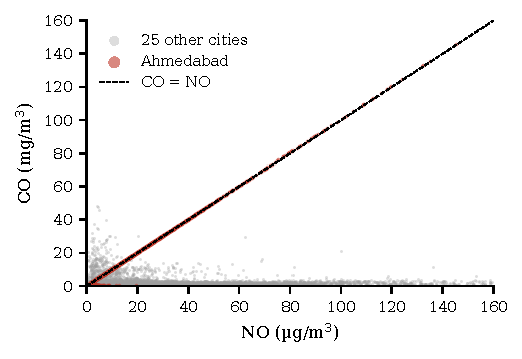
\includegraphics[width=\columnwidth]{fig1_ahmedabad_co_no.pdf}
\caption{Daily CO against NO. Ahmedabad's points lie on the identity line, showing that the
CO column copies NO; other cities show no such pattern.}
\label{fig:coNO}
\end{figure}

\subsection{Unseen cities}
Eight cities enter the record only in 2019--2020 (Aizawl, Bhopal, Chandigarh, Coimbatore,
Ernakulam, Guwahati, Kochi, Shillong; 2,036 test rows). They act as an out-of-sample-city
check.

%=====================================================================
\section{Methods}
\subsection{Deterministic baselines}
\textbf{B1, CPCB formula.} The national sub-index tables~\cite{cpcb2014} are applied to each
day's mean concentrations and the maximum is taken. The CPCB defines the index on trailing
windows (24-h means; 8-h maxima for CO and O$_3$), so daily means cannot reproduce it exactly.
\textbf{B2, recalibrated formula} fits $\text{AQI}\approx a\,\text{B1}+b$ on 2015--2018.
\textbf{B3, two-day formula.} Each concentration is replaced by $(1-w)c_t+w\,c_{t-1}$ before
B2 is applied, and the nitrogen sub-index uses NO$_2$ or NO$_x$. The source, $w$, $a$ and $b$
are chosen on 2015--2018 only (selected: NO$_x$, $w=0.40$, $a=0.94$, $b=17.0$). A trailing
window that reaches into the previous day explains why yesterday's readings help.

\subsection{Learned models}
We train Random Forest~\cite{breiman2001}, XGBoost~\cite{chen2016xgboost},
LightGBM~\cite{ke2017lightgbm} and CatBoost~\cite{prokhorenkova2018catboost} on two feature
sets. \textbf{S} has the same-day readings of PM$_{2.5}$, PM$_{10}$, NO, NO$_2$, NO$_x$, NH$_3$,
CO, SO$_2$ and O$_3$. \textbf{SL} adds the same nine readings from the previous calendar day,
which are available at estimation time. Missing inputs are handled natively by each library,
with no imputation. Each model gets the same budget of 20 random-search
configurations~\cite{bergstra2012random}, fitted on 2015--2017 and scored by 2018 MAE; boosting
rounds are set by early stopping (patience 100). The selected configuration is refit on
2015--2018 with five seeds, and we report the mean and SD over seeds. Search spaces and the
selected values are released with the code.

\subsection{Outage protocol}\label{sec:protocol}
To create ground truth for missing inputs, we use the 8,003 test rows (22 cities) on which every
input is observed today, so the target is unchanged by masking. An outage of length
$L\in\{1,3,7\}$ removes an analyser's readings for days $t-L+1,\dots,t$; for $L\ge2$ the
previous-day input is lost as well. NO, NO$_2$ and NO$_x$ come from one chemiluminescence
analyser and are removed together. Scenarios mask PM$_{2.5}$, PM$_{10}$, CO, the NO$_x$
analyser, both PM analysers, or the row's \emph{dominant} analyser (the one that sets the
formula AQI), which is the hardest single failure.

The reference is \textbf{Formula+LOCF}: B3 with each missing reading replaced by the
analyser's last available value (last observation carried forward, from day $t-L$ or earlier,
within 30 days). We compare it with B3 on the remaining analysers (\textbf{Formula-drop}) and
with SL models in three variants: trained normally and given NaN; trained with one extra copy
of each row in which a random analyser is masked (\textbf{-aug}); and trained with copies whose
masked analyser is filled with its last reading 1, 3 or 7 days old plus an input giving that
age in days (\textbf{-stale}). The stale variant receives the last reading and its true age at
test time. Models are LightGBM and Random Forest with the configurations selected above.

\subsection{Statistics}
Errors on the same day across cities are correlated, so confidence intervals for paired MAE
differences use a date-block bootstrap~\cite{kunsch1989bootstrap}: whole test days are
resampled (2,000 replicates), and errors are averaged over seeds first. We report
differences and 95\% intervals instead of $p$-values. We also report the share of days placed
in the correct CPCB category (Good to Severe), which is what an advisory communicates.

%=====================================================================
\section{Results}
\subsection{Complete inputs}\label{sec:complete}
Table~\ref{tab:main} shows the benchmark. The raw formula on daily means is biased low
($-8.1$ points), reflecting the gap between daily means and trailing windows. Recalibration
shrinks the bias to $+3.9$, and adding yesterday's readings (B3) cuts MAE from 16.96 to 12.26.

The same-day models, the setup of the original study, lie within 0.6 points of each other
(MAE 16.0--16.6) and are \emph{worse} than B3 by 3.8--4.3 points (all 95\% CIs exclude zero).
Previous-day inputs improve every model by 4.2--4.6 points. With those inputs, Random Forest
and LightGBM beat B3's MAE by 0.47 [0.24, 0.69] and 0.42 [0.19, 0.64] points, while XGBoost
and CatBoost are indistinguishable from it. On RMSE, B3 is the best method in the table. A
four-parameter formula therefore captures nearly all of what the ensembles learn when every
analyser reports. Seed SD is at most 0.16 MAE points,
small next to the gaps that matter here.

\begin{table}[t]
\centering
\caption{Test performance with complete inputs (1 Jan 2019--1 Jul 2020, Ahmedabad excluded,
$n=10{,}882$). ML rows: mean over 5 seeds (MAE SD $\le0.16$). Band: share of days in the
correct CPCB category.}
\label{tab:main}
\setlength{\tabcolsep}{4pt}
\begin{tabular}{@{}llcccc@{}}
\toprule
 & Method & MAE & RMSE & $R^2$ & Band \\
\midrule
\multirow{3}{*}{\rotatebox{90}{\scriptsize Formula}}
 & B1 CPCB formula (same day)     & 18.33 & 27.82 & 0.890 & 0.737 \\
 & B2 recalibrated (same day)     & 16.96 & 25.39 & 0.908 & 0.764 \\
 & B3 two-day recalibrated        & 12.26 & \textbf{18.31} & \textbf{0.952} & 0.820 \\
\midrule
\multirow{4}{*}{\rotatebox{90}{\scriptsize Same day}}
 & Random Forest & 16.01 & 25.10 & 0.910 & 0.762 \\
 & XGBoost       & 16.58 & 24.47 & 0.915 & 0.763 \\
 & LightGBM      & 16.45 & 24.78 & 0.913 & 0.755 \\
 & CatBoost      & 16.51 & 24.32 & 0.916 & 0.757 \\
\midrule
\multirow{4}{*}{\rotatebox{90}{\scriptsize + prev.\ day}}
 & Random Forest & \textbf{11.78} & 19.56 & 0.946 & \textbf{0.825} \\
 & XGBoost       & 12.24 & 19.34 & 0.947 & 0.817 \\
 & LightGBM      & 11.83 & 18.54 & 0.951 & 0.820 \\
 & CatBoost      & 12.30 & 18.37 & \textbf{0.952} & 0.819 \\
\bottomrule
\end{tabular}
\end{table}

\subsection{Where the learned model loses}
Breaking down the best model (Random Forest, SL) against B3 shows where the small average
gain comes from (Table~\ref{tab:break}). ML is better in the Satisfactory, Moderate and Poor
categories, which hold 85\% of days, but worse in Good, Very Poor and Severe. The last two
are rare (6\% of test days). On the eight cities absent from training, ML is
\emph{worse} than the formula (13.78 vs 11.42), while the formula, which has no
city-specific parameters, transfers unchanged. Comparing equal calendar windows removes the
seasonal confound of the original study. ML's margin is largest from 25 Mar to 1 Jul 2019
(12.26 vs 14.18). It shrinks to 0.4 points over the same window in 2020, the lockdown period
\cite{sharma2020covid}, when mean AQI fell from 124 to 82. In early 2019 the formula is
marginally ahead.

\begin{table}[t]
\centering
\caption{MAE of the best ML model (Random Forest, SL) and the two-day formula (B3) by subgroup.}
\label{tab:break}
\setlength{\tabcolsep}{4pt}
\begin{tabular}{@{}lrrcc@{}}
\toprule
Subgroup & $n$ & Mean AQI & ML & B3 \\
\midrule
Cities seen in training   & 8,846 & 132.1 & \textbf{11.30} & 12.45 \\
Cities unseen in training & 2,036 & 100.9 & 13.78 & \textbf{11.42} \\
\midrule
Good (0--50)            &   933 &  39.9 & 11.49 & \textbf{10.55} \\
Satisfactory (51--100)  & 4,469 &  76.3 & \textbf{8.89} & 9.45 \\
Moderate (101--200)     & 3,841 & 134.4 & \textbf{12.04} & 13.34 \\
Poor (201--300)         &   976 & 245.6 & \textbf{19.04} & 21.06 \\
Very Poor (301--400)    &   536 & 336.2 & 13.89 & \textbf{9.73} \\
Severe ($>$400)         &   127 & 466.8 & 41.23 & \textbf{33.84} \\
\midrule
1 Jan--24 Mar 2019      & 1,425 & 188.5 & 14.03 & \textbf{13.91} \\
1 Jan--24 Mar 2020      & 1,907 & 139.3 & \textbf{11.15} & 11.66 \\
25 Mar--1 Jul 2019      & 1,688 & 124.4 & \textbf{12.26} & 14.18 \\
25 Mar--1 Jul 2020      & 2,296 &  82.2 & \textbf{11.19} & 11.61 \\
\bottomrule
\end{tabular}
\end{table}

\subsection{Analyser outages}\label{sec:outage}
Which formula strategy is better depends on the outage length. Filling with the last reading
is best for one-day outages, but by day three a stale reading is often worse than simply
dropping the analyser (e.g., PM$_{2.5}$ out for three days: MAE 23.00 with the last reading vs
19.60 when dropped). We therefore compare the learned model with whichever formula strategy
has the lower MAE in each scenario. This choice is made on the test data and favours the
formula. As the learned model we pre-specify LightGBM-stale, the only variant that is trained
on the conditions it meets at test time. Table~\ref{tab:outage} and Fig.~\ref{fig:outage}
report the results.

\begin{table}[t]
\centering
\caption{Outages: MAE of LightGBM-stale minus the better formula strategy, with 95\%
date-block bootstrap CIs (negative means ML is better). $n=8{,}003$ complete-input test rows.}
\label{tab:outage}
\setlength{\tabcolsep}{3pt}
\begin{tabular}{@{}lccc@{}}
\toprule
Analyser(s) out & 1 day & 3 days & 7 days \\
\midrule
Dominant    & $\mathbf{-1.97}$ {\scriptsize[$-2.30$,$-1.64$]} & $\mathbf{-6.34}$ {\scriptsize[$-6.88$,$-5.77$]} & $\mathbf{-6.02}$ {\scriptsize[$-6.70$,$-5.38$]} \\
PM$_{2.5}$+PM$_{10}$ & $\mathbf{-1.04}$ {\scriptsize[$-1.35$,$-0.72$]} & $\mathbf{-3.46}$ {\scriptsize[$-3.94$,$-3.02$]} & $\mathbf{-4.91}$ {\scriptsize[$-5.46$,$-4.37$]} \\
PM$_{2.5}$  & $\mathbf{-1.32}$ {\scriptsize[$-1.61$,$-1.02$]} & $\mathbf{-1.03}$ {\scriptsize[$-1.75$,$-0.30$]} & $-0.29$ {\scriptsize[$-0.97$,$+0.38$]} \\
PM$_{10}$   & $\mathbf{-0.99}$ {\scriptsize[$-1.31$,$-0.66$]} & $-0.28$ {\scriptsize[$-0.80$,$+0.24$]} & $+0.77$ {\scriptsize[$+0.23$,$+1.30$]} \\
CO          & $-0.02$ {\scriptsize[$-0.27$,$+0.24$]} & $+0.08$ {\scriptsize[$-0.17$,$+0.34$]} & $+0.10$ {\scriptsize[$-0.16$,$+0.35$]} \\
NO$_x$ analyser & $-0.05$ {\scriptsize[$-0.31$,$+0.21$]} & $+0.25$ {\scriptsize[$-0.02$,$+0.52$]} & $+0.34$ {\scriptsize[$+0.08$,$+0.61$]} \\
\bottomrule
\end{tabular}
\end{table}

\begin{figure}[t]
\centering
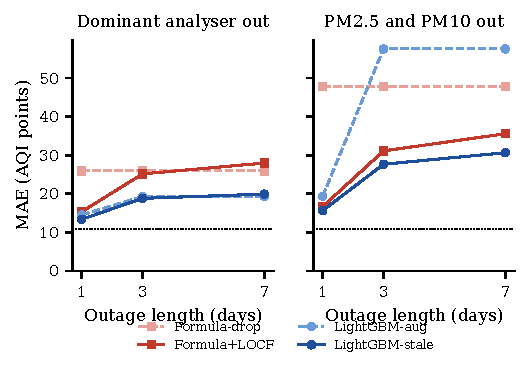
\includegraphics[width=\columnwidth]{fig3_outage.pdf}
\caption{MAE against outage length for the two formula strategies and two learned variants.
The dotted line is the error with no outage.}
\label{fig:outage}
\end{figure}

When the failed analyser is the one setting the index, dropping it
makes the formula report the \emph{second}-highest sub-index, and a stale value misses the
day's change. The learned model instead infers the missing level from correlated analysers
(PM$_{2.5}$ from PM$_{10}$, CO and NO$_x$, and the reverse), cutting error by about 2 points
for one-day outages and by about 6 points for longer ones. The same holds when both PM
analysers fail; in that case the formula's output is not even a valid CPCB AQI, because no
PM reading remains. When an analyser that rarely sets the index fails (CO, NO$_x$), both
approaches are within 0.35 points of each other, with the formula slightly ahead for
week-long NO$_x$ outages. For long single-PM outages the advantage
disappears, and for PM$_{10}$ out for a week the formula is better by 0.77 points. The
dominant analyser is PM$_{10}$ on 56\% of these days and PM$_{2.5}$ on 27\%, so it is usually,
but not always, a PM analyser.

Training on the failure mode matters. The NaN-augmented model, which saw only single-analyser
gaps, collapses when both PM analysers are missing for three or more days (MAE 57.6, worse
than the formula). The stale variant, which always sees a reading plus its age, degrades
gradually (MAE 15.6 to 30.7 from 1 to 7 days). Random Forest-stale follows the same pattern
with smaller gains, and loses to the formula by 1.37 [0.62, 2.12] points when PM$_{2.5}$ is
out for a week.

\subsection{Attributions and the Ahmedabad effect}
For the same-day CatBoost model we sum the mean absolute TreeSHAP value of each analyser
(NO, NO$_2$ and NO$_x$ as one group) over the test set. We compare these shares with how
often each analyser actually sets the formula AQI, which is ground truth for this task
(Fig.~\ref{fig:shap}). With Ahmedabad in the data, CO receives 20.0\% of the attribution and
the NO$_x$ group 16.1\%, close to the 22\% for CO reported in the original study with a
different feature set. Without Ahmedabad these fall to 9.9\% and 8.5\%, and CO's share is close
to how often it sets the index (11.1\% of test days). The duplicated column, not atmospheric chemistry, had inflated CO's importance.

Even on clean data, SHAP ranks the analysers differently from the formula. PM$_{10}$ sets the
index on 48.7\% of days but receives 20.7\% of the attribution, while PM$_{2.5}$ receives 50.2\%
against a dominance of 32.8\%. The two are strongly correlated, and the model can recover
either from the other, so the credit is split according to the fitted trees rather than the
index definition~\cite{aas2021shapley}. Attribution rankings for this task therefore
describe the model, not which pollutant drives the AQI.

\begin{figure}[t]
\centering
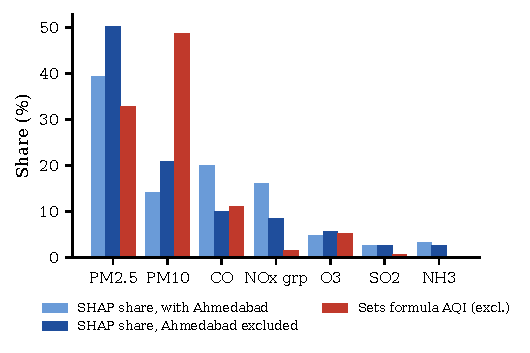
\includegraphics[width=\columnwidth]{fig2_shap_vs_dominant.pdf}
\caption{Share of mean $|$SHAP$|$ per analyser for same-day CatBoost with and without
Ahmedabad, against the share of test days on which each analyser sets the formula AQI.}
\label{fig:shap}
\end{figure}

\textit{Sensitivity: keeping Ahmedabad.} Rerunning the full benchmark with Ahmedabad
(11,410 test rows) reverses the same-day comparison: Random Forest beats the two-day formula
by 1.15 [0.52, 1.82] points, and the best previous-day model by 5.72 points. The whole
reversal comes from Ahmedabad's 528 test rows (formula 123.4, Random Forest 88.8). On the
other 25 cities, the formula (15.75) still beats same-day Random Forest (16.21) and CatBoost
(16.77), even though both were trained with Ahmedabad included. Learned models fit the
corrupted mapping better than the formula can, which is not a reason to prefer them.

%=====================================================================
\section{Discussion and Limitations}
\textit{Implications.} Reports of $R^2\approx0.9$ for same-day AQI regression should be read
against the formula: in our test period a four-parameter formula is better than every same-day
ensemble. The useful role for learning is narrower but real. A station can publish the
two-day formula when all analysers report and switch to a learned model when the
analyser that usually sets the index is down. The model must be trained on the failure mode it
will face; generic missing-value handling is not enough.

\textit{Limitations.} (i)~Only daily means are available, so neither the formula nor the models
see the trailing windows that define the index; hourly data would tighten both.
(ii)~Outages are simulated on complete-input days and are random with respect to the
pollution level; real outages may correlate with weather or with high-pollution episodes.
(iii)~The dominant-analyser scenario chooses the masked analyser using full information, so
it is a stress test rather than an estimate of average risk. The stale model was also trained
on the same outage lengths (1, 3, 7 days) that we test. (iv)~One out-of-time window
(2019--mid-2020) is evaluated, and it includes the COVID-19 lockdown. (v)~Excluding Ahmedabad
is a decision made after inspecting the data; we give the criterion and the full-data
results. Other defects remain, such as zero-valued CO in Mumbai and multi-day constant
readings. (vi)~There are no meteorological inputs, and the learned model transfers to new
cities worse than the formula. (vii)~SHAP describes the fitted model, not atmospheric
causation~\cite{lundberg2020treeshap}.

%=====================================================================
\section{Conclusion}
On the CPCB \texttt{city\_day} data, the question ``can ML estimate the AQI?'' has a
deceptively easy answer, because the index is a formula of the inputs. Measured against that
formula, same-day tree ensembles lose. With previous-day inputs they gain only about half
a point, and they transfer worse to new cities. Their clear value appears when the analyser
that sets the index fails: with training that mimics stale readings, LightGBM reduces error
by about 2 points for one-day outages and about 6 points for longer ones, relative to the
better of two formula strategies. A one-city column duplication in a widely shared dataset was
enough to distort both accuracy and attributions, so we recommend formula baselines and
data audits as standard practice for this task. Future work should use hourly data, outages
observed in real station logs, and meteorological inputs.

\section*{Data and Code Availability}
The dataset is public~\cite{rao2020kaggle}. Scripts that reproduce the audit, the benchmark,
the outage experiment, and every table and figure, including search spaces, selected
hyperparameters and seeds, are available at \tbd{[anonymised repository URL]}.

\bibliographystyle{IEEEtran}
\bibliography{references}

\end{document}
